\chapter{Einleitung}

\section{Definition eines verteilten Systems}

In der Literatur findet man viele verschiedene Definitionen eins verteiltes Systems. Vieler dieser Definitionen unterschieden sich untereinander, so dass es schwerf\"{a}llt eine Definition zu finden, die als Alleinige als die Richtige gilt. Andrew Tanenbaum und Marten van Steen haben f\"{u}r die Beschreibung eins verteilten Systems die Folgende lockere Charakterisierung formuliert:

\cite{Tanenbaum} \textit{``Ein verteiltes System ist eine Menge voneinander unabh\"{a}ngiger Computer, die dem Benutzer wie ein einzelnes, koh\"{a}rentes System erscheinen''}

\begin{figure}[htbp]
	\centering
	\fbox{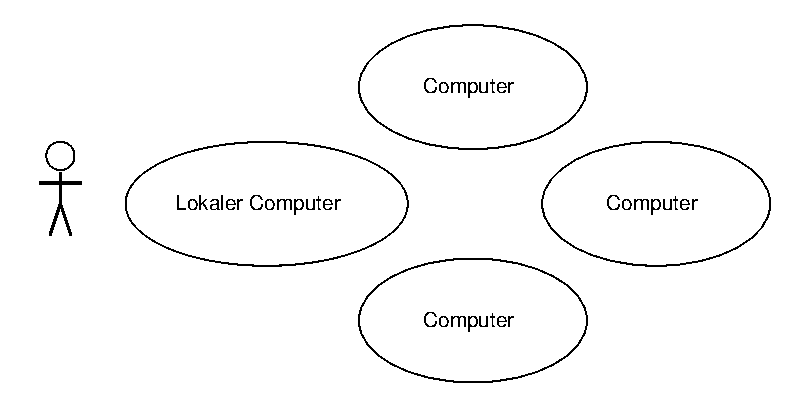
\includegraphics{images/verteiltes-system}}
	\caption{Ein verteiltes System bestehend aus 4 Computern}
	\label{fig:VerteiltesSystem}
\end{figure}

Demnach erscheint dem Benutzer ein aus mehreren Computern bestehendes verteiltes System wie ein System, welches lediglich aus einem einzigen Computer besteht. Der Benutzer muss sich nur mit dem lokalen vor ihm befindenden Computer auseinandersetzen (Abbildung \ref{fig:VerteiltesSystem}). Die Software des lokalen Computer stellt die reibungslose Kommunikation mit anderen Computern des verteilten Systems sicher und der Benutzer muss sich darum nicht selbst k\"{u}mmern.

\section{Motivation}

In dieser Diplomarbeit betrachten wir ein verteiltes System jedoch von einer anderen Perspektive. Wir nehmen nicht die Sichtweise eines Endbenutzers ein, sondern wollen die grundlegenen Funktionsweisen, wie unabh\"{a}ngige Computer in einem verteilten System miteinander agieren, verstehen. Es sollen alle relevanten Ereignisse eines verteilten Systems sichtbar und verst\"{a}ndlich repr\"{a}sentiert werden.

Um dieses Ziel zu erreichen wurde ein Simulator entwickelt, der dies erm\"{o}glicht. Der Simulator wurde insbesondere f\"{u}r Lehr- und Lernzwecke entwickelt. Er inspiriert auch die Entwicklung eigener verteilter Systeme.

